\documentclass[../lecture-notes.tex]{subfiles}

\begin{document}

\subsection{Schnorr's Identification Protocol}

To better illustrate the Fiat-Shamir Transformation in practice, let us consider one of the most basic Sigma protocols: non-interactive Schnorr Identification Protocol. It is a simple and elegant protocol that allows one party to prove to another party that it knows a discrete logarithm of a given element. It is also quite straightforward to generalize it to a signature scheme.

Let us formalize it using theory from \Cref{section:relations_and_languages}. Suppose $\mathbb{G}$ is a cyclic group of order $q$ with a generator $g$. Then, the relation and language being considered are:
\begin{equation*}
    \mathcal{R} = \{(u, \alpha) \in \mathbb{G} \times \mathbb{Z}_q: u = g^{\alpha}\}, \; \mathcal{L}_{\mathcal{R}} = \{u \in \mathbb{G}: \exists \alpha \in \mathbb{Z}_q: u = g^{\alpha}\}
\end{equation*}

Now, suppose prover $\mathcal{P}$ has a valid statement and a witness $(u,\alpha) \in \mathcal{R}$ and he wants to convince the verifier $\mathcal{V}$ that he knows the witness $\alpha$ to the public statement $u$ (that is, we are building the proof of knowledge). Well, the easiest way how to proceed is simply giving $\alpha$ to $\mathcal{V}$, but this is obviously not what we want. Instead, the Schnorr protocol allows $\mathcal{P}$ to prove the knowledge of $\alpha$ without revealing it. 

First, let us start with the interactive version of the protocol. 

\begin{definition}
    \textbf{The Schnorr interactive identification protocol} $\Pi_{\text{Sch}} = (\mathsf{Gen}, \mathcal{P}, \mathcal{V})$ with a generation function $\mathsf{Gen}$ and prover $\mathcal{P}$ and verifier $\mathcal{V}$ is defined as follows:
    \begin{itemize}
        \item $\mathsf{Gen}(1^{\lambda})$: As with most public-key cryptosystems, we take $\alpha \xleftarrow{R} \mathbb{Z}_q$ and $u \gets g^{\alpha}$. We output the \textit{verification key} as $\mathsf{vk} := u$, and the \textit{secret key} as $\mathsf{sk} := \alpha$.
        \item The protocol between $(\mathcal{P},\mathcal{V})$ is run as follows:
        \begin{itemize}
            \item $\mathcal{P}$ computes $r \gets \mathbb{Z}_q^{\times}, a \gets g^{r}$ and sends $a$ to $\mathcal{V}$.
            \item $\mathcal{V}$ sends a random challenge $e \xleftarrow{R} \mathbb{Z}_q$ to $\mathcal{P}$.
            \item $\mathcal{P}$ computes $\sigma \gets r + \alpha e \in \mathbb{Z}_q$ and sends $\sigma$ to $\mathcal{V}$.
            \item $\mathcal{V}$ accepts if $g^{\sigma} = a \cdot u^e$, otherwise it rejects.
        \end{itemize}
    \end{itemize}

    This protocol is illustrated in \Cref{fig:interactive_schnorr}. 
\end{definition}

\begin{figure}[H]
    \centering
    \begin{tikzpicture}
        \node[inner sep=0pt, align=center] (prover) {
\includegraphics[width=1.25cm]{lectures/images/common/prover.png}\\Prover $\mathcal{P}$};
        \node[inner sep=0pt, align=center, right=5cm of prover] (verifier) {
\includegraphics[width=1.25cm]{lectures/images/common/verifier.png}\\Verifier $\mathcal{V}$};

        \draw [dashed,line width=0.3mm] ([yshift=-0.5cm]prover.south) -- ([yshift=-9cm]prover.south);
        \draw [dashed,line width=0.3mm] ([yshift=-0.5cm]verifier.south) -- ([yshift=-9cm]verifier.south);

        \node[align=center,fill=white!5,thick,below=0.5cm of prover](prover-setup){
        \noindent\rule{3.5cm}{0.8pt}\\
        $r \xleftarrow{R} \mathbb{Z}_q^{\times}$ \\
        $a \gets g^r$ \\
        \noindent\rule{3.5cm}{0.8pt}};

        \draw[-{Stealth[length=3mm]},line width=0.4mm] ([yshift=-3cm]prover.south) coordinate (l2)--(l2-|verifier) node[midway, above=0mm]{Send $a$};

        \node[align=center,fill=white!5,thick,below=3.5cm of verifier](verifier-choice){
        \noindent\rule{3.5cm}{0.8pt}\\
        $e \xleftarrow{R} \mathbb{Z}_q$ \\
        \noindent\rule{3.5cm}{0.8pt}};

        \draw[-{Stealth[length=3mm]},line width=0.4mm] ([yshift=-5.5cm]verifier.south) coordinate (l2)--(l2-|prover) node[midway, above=0mm]{Send $e$};

        \node[align=center,fill=white!5,thick,below=6.0cm of prover](prover-setup){
        \noindent\rule{3.5cm}{0.8pt}\\
        Compute $\sigma \gets r + \alpha e \in \mathbb{Z}_q$\\
        \noindent\rule{3.5cm}{0.8pt}};

        \draw[-{Stealth[length=3mm]},line width=0.4mm] ([yshift=-8cm]prover.south) coordinate (l2)--(l2-|verifier) node[midway, above=0mm]{Send $\sigma$};

        \node[align=center,fill=white!5,thick,below=8.5cm of verifier](verifier-choice){
        \noindent\rule{3.5cm}{0.8pt}\\
        Verify $g^{\sigma} = a \cdot u^e$ \\
        \noindent\rule{3.5cm}{0.8pt}};
    \end{tikzpicture}

    \caption{The interactive Schnorr protocol between prover $\mathcal{P}$ and verifier $\mathcal{V}$ for proof of knowledge of discrete logarithm relation.}
    \label{fig:interactive_schnorr}
\end{figure}

\begin{definition}
    An interaction between $\mathcal{P}$ and $\mathcal{V}$ produces the so-called \textbf{conversation} $(a,e,\sigma) \in \mathbb{G} \times \mathbb{Z}_q \times \mathbb{Z}_q$. We call such a conversation an \textbf{accepting conversation} if $\mathcal{V}$ accepts the proof.
\end{definition}

\begin{example}
    In case of a Schnorr protocol, the accepting conversation is such that $g^{\sigma} = a \cdot u^e$.
\end{example}

Now, one can prove the following theorem.
\begin{theorem}
    The Schnorr protocol $\Pi_{\text{Sch}}$ is complete, sound, and (honest verifier) zero-knowledge proof of knowledge.
\end{theorem}

\textbf{Proof.} We are not going to prove the zero-knowledge and soundness properly, but completeness and proof of knowledge are quite straightforward to show.

\begin{itemize}
    \item \textbf{Completeness.} Just observe that $g^{\sigma} = g^{r+\alpha e} = g^r(g^{\alpha})^e = a \cdot u^e$.
    \item \textbf{Proof of Knowledge.} To prove that the protocol is a proof of knowledge, we need to construct an extractor $\mathcal{E}^{\mathcal{P}}$. We construct it as follows:
    \begin{enumerate}
        \item Extractor runs the prover and gets $a$, $e$, and $\sigma$ as a response.
        \item Extractor rewinds back to the verifier's challenge step, generates a new challenge $e' \xleftarrow{R} \mathbb{Z}_q$ and gets new prover's response $\sigma'$ (for the same prover's randomness $r$).
        \item Extractor outputs the witness $\alpha \gets (\sigma - \sigma')(e - e')^{-1}$.
    \end{enumerate}
    The reason why this works is following: notice that $g^{\sigma} = a \cdot u^{e}, g^{\sigma'} = a \cdot u^{e'}$. Therefore, by dividing former by latter, we obtain $g^{\sigma - \sigma'} = u^{e - e'} = g^{\alpha(e-e')}$. It immediately follows that $\alpha = (\sigma - \sigma')(e - e')^{-1}$.
\end{itemize}

\vspace{10px}

\begin{remark}
    Before considering how to make such protocol non-interactive correctly, suppose that we instead do the following: after interaction with the verifier, the prover publishes the conversation as a proof of knowledge. Would that be a valid non-interactive proof? In other words, can we convince the independent observer of the interaction that the prover knows the witness? The answer is no (and it is generally so for any interactive protocol). The reason why is that the prover can first sample randomly $e,\sigma \xleftarrow{R} \mathbb{Z}_q$, compute $a \gets g^{\sigma}/u^e$ and simply publish $(a,e,\sigma)$ as a proof. This is a valid conversation since $g^{\sigma} = a \cdot u^{e} = (g^{\sigma}/u^e) \cdot u^e$ and thus the observer would be convinced that the prover knows the witness. However, the prover might not know the witness at all!

    Therefore, either (1) the prover needs to get a challenge $e$ \textbf{before} he commits to the value $\sigma$, or (2) challenge must be randomized. Otherwise, he can precompute $\sigma$ and publish it as a proof (or simply make a deal with the verifier to fool the observer). 
\end{remark}

Now, notice that the provided protocol is a public-coin protocol. Therefore, we can apply the Fiat-Shamir transformation to make it non-interactive. Suppose we have a random oracle $\mathcal{O}_{\text{R}}: \mathbb{G} \times \mathbb{G} \to \mathbb{Z}_q$:
\begin{enumerate}
    \item The prover $\mathcal{P}$ computes $r \gets \mathbb{Z}_q^{\times}, a \gets g^{r}$ and sends $a$ to the Fiat-Shamir Channel.
    \item The Fiat-Shamir channel responds with the challenge $e \gets \mathcal{O}_{\text{R}}(u,a)$.
    \item The prover $\mathcal{P}$ computes $\sigma \gets r + \alpha e$ and sends $\sigma$ to the Fiat-Shamir Channel.
    \item The Fiat-Shamir channel outputs the proof $\pi = (a,e,\sigma)$, which the verifier can check via previously mentioned equation $g^{\sigma} = a \cdot u^e$.
\end{enumerate}

Now, notice that $e$ might not be included in the proof since the verifier can compute it by himself. Therefore, the final proof $\pi$ can be reduced to $(a,\sigma) \in \mathbb{G} \times \mathbb{Z}_q$ and its computation does not need any interaction with the verifier. Moreover, it is still complete, sound, and proof of knowledge due to the Fiat-Shamir transformation. It is also (not easy to prove) zero-knowledge.

\subsection{Schnorr's Signature Scheme}

Now, turning the Schnorr's Identification Protocol into a signature scheme is quite straightforward. The only modification to the non-interactive proof described in the previous section is that we include the message $m \in \mathcal{M}$ instead of our statement $u \in \mathbb{G}$ in the computation of the challenge $e$. Additionally, suppose we use the hash function $H$ as a random oracle from the previous section. Now, let us give a formal definition.

\begin{definition}
    The Schnorr Signature Scheme is $\Sigma_{\text{Sch}} = (\mathsf{Gen}, \mathsf{Sign}, \mathsf{Verify})$, where:
    \begin{itemize}
        \item $\mathsf{Gen}(1^{\lambda})$: We take $\alpha \xleftarrow{R} \mathbb{Z}_q$ and $u \gets g^{\alpha}$. The \textit{public key} is $\mathsf{pk} := u$, while the \textit{secret key} as $\mathsf{sk} := \alpha$.
        \item $\mathsf{Sign}(m,\mathsf{sk})$: The signer computes $r \gets \mathbb{Z}_q^{\times}, a \gets g^{r}, e \gets H(m, a), \sigma \gets r + \alpha e$ and outputs the signature $(a,\sigma)$.
        \item $\mathsf{Verify}((a, \sigma), m,\mathsf{pk})$: The verifier checks if $g^{\sigma} = a \cdot u^e$ for $e \gets H(m, a)$.
    \end{itemize}
\end{definition}

\begin{remark}
    Typically, one also uses a so-called ``\textit{key-prefixed}'' variant of the scheme, where the challenge $e$ is computed as $e \gets H(\mathsf{pk}, m, a)$ for a random oracle $H: \mathbb{G} \times \mathcal{M} \times \mathbb{G} \to \mathbb{Z}_q$. It was argued that such variant has a better multi-user security bound than the classical one.
\end{remark}

\subsection{Sigma Protocols}

Now, the Schnorr Protocol is just one of the many examples of a so-called \textbf{Sigma Protocol}. Sigma protocols are a class of interactive proof systems that are used to prove the knowledge of a witness to a statement. They are quite general and can be used to prove the knowledge of a witness to any effective relation $\mathcal{R} \subseteq \mathcal{X} \times \mathcal{W}$, where $\mathcal{X}$ is the set of public statements and $\mathcal{W}$ is the set of witnesses. Let us define them formally.

\begin{definition}
    Let $\mathcal{R} \subset \mathcal{X} \times \mathcal{W}$ be an effective relation. A \textbf{Sigma protocol} for $\mathcal{R}$ is an interactive protocol $(\mathcal{P}, \mathcal{V})$ that satisfies the following properties:
    \begin{itemize}
        \item In the beginning, $\mathcal{P}$ computes a \textbf{commitment} $a$ and sends it to $\mathcal{V}$.
        \item $\mathcal{V}$ chooses a random \textbf{challenge} $c \in \mathcal{C}$ from the challenge space $\mathcal{C}$ and sends it to $\mathcal{P}$.
        \item Upon receiving $c$, $\mathcal{P}$ computes the response $z$ and sends it to $\mathcal{V}$.
        \item $\mathcal{V}$ outputs either $\mathsf{accept}$ or $\mathsf{reject}$ based on the conversation transcript $(a,c,z)$.
    \end{itemize}
\end{definition}

\begin{remark}
    The name ``Sigma'' protocol comes from the fact that the ``shape'' of the message flow vaguely resembles the Greek letter $\Sigma$: see \Cref{fig:sigma_protocol_illustration}.
\end{remark}

\begin{figure}[H]
    \centering
    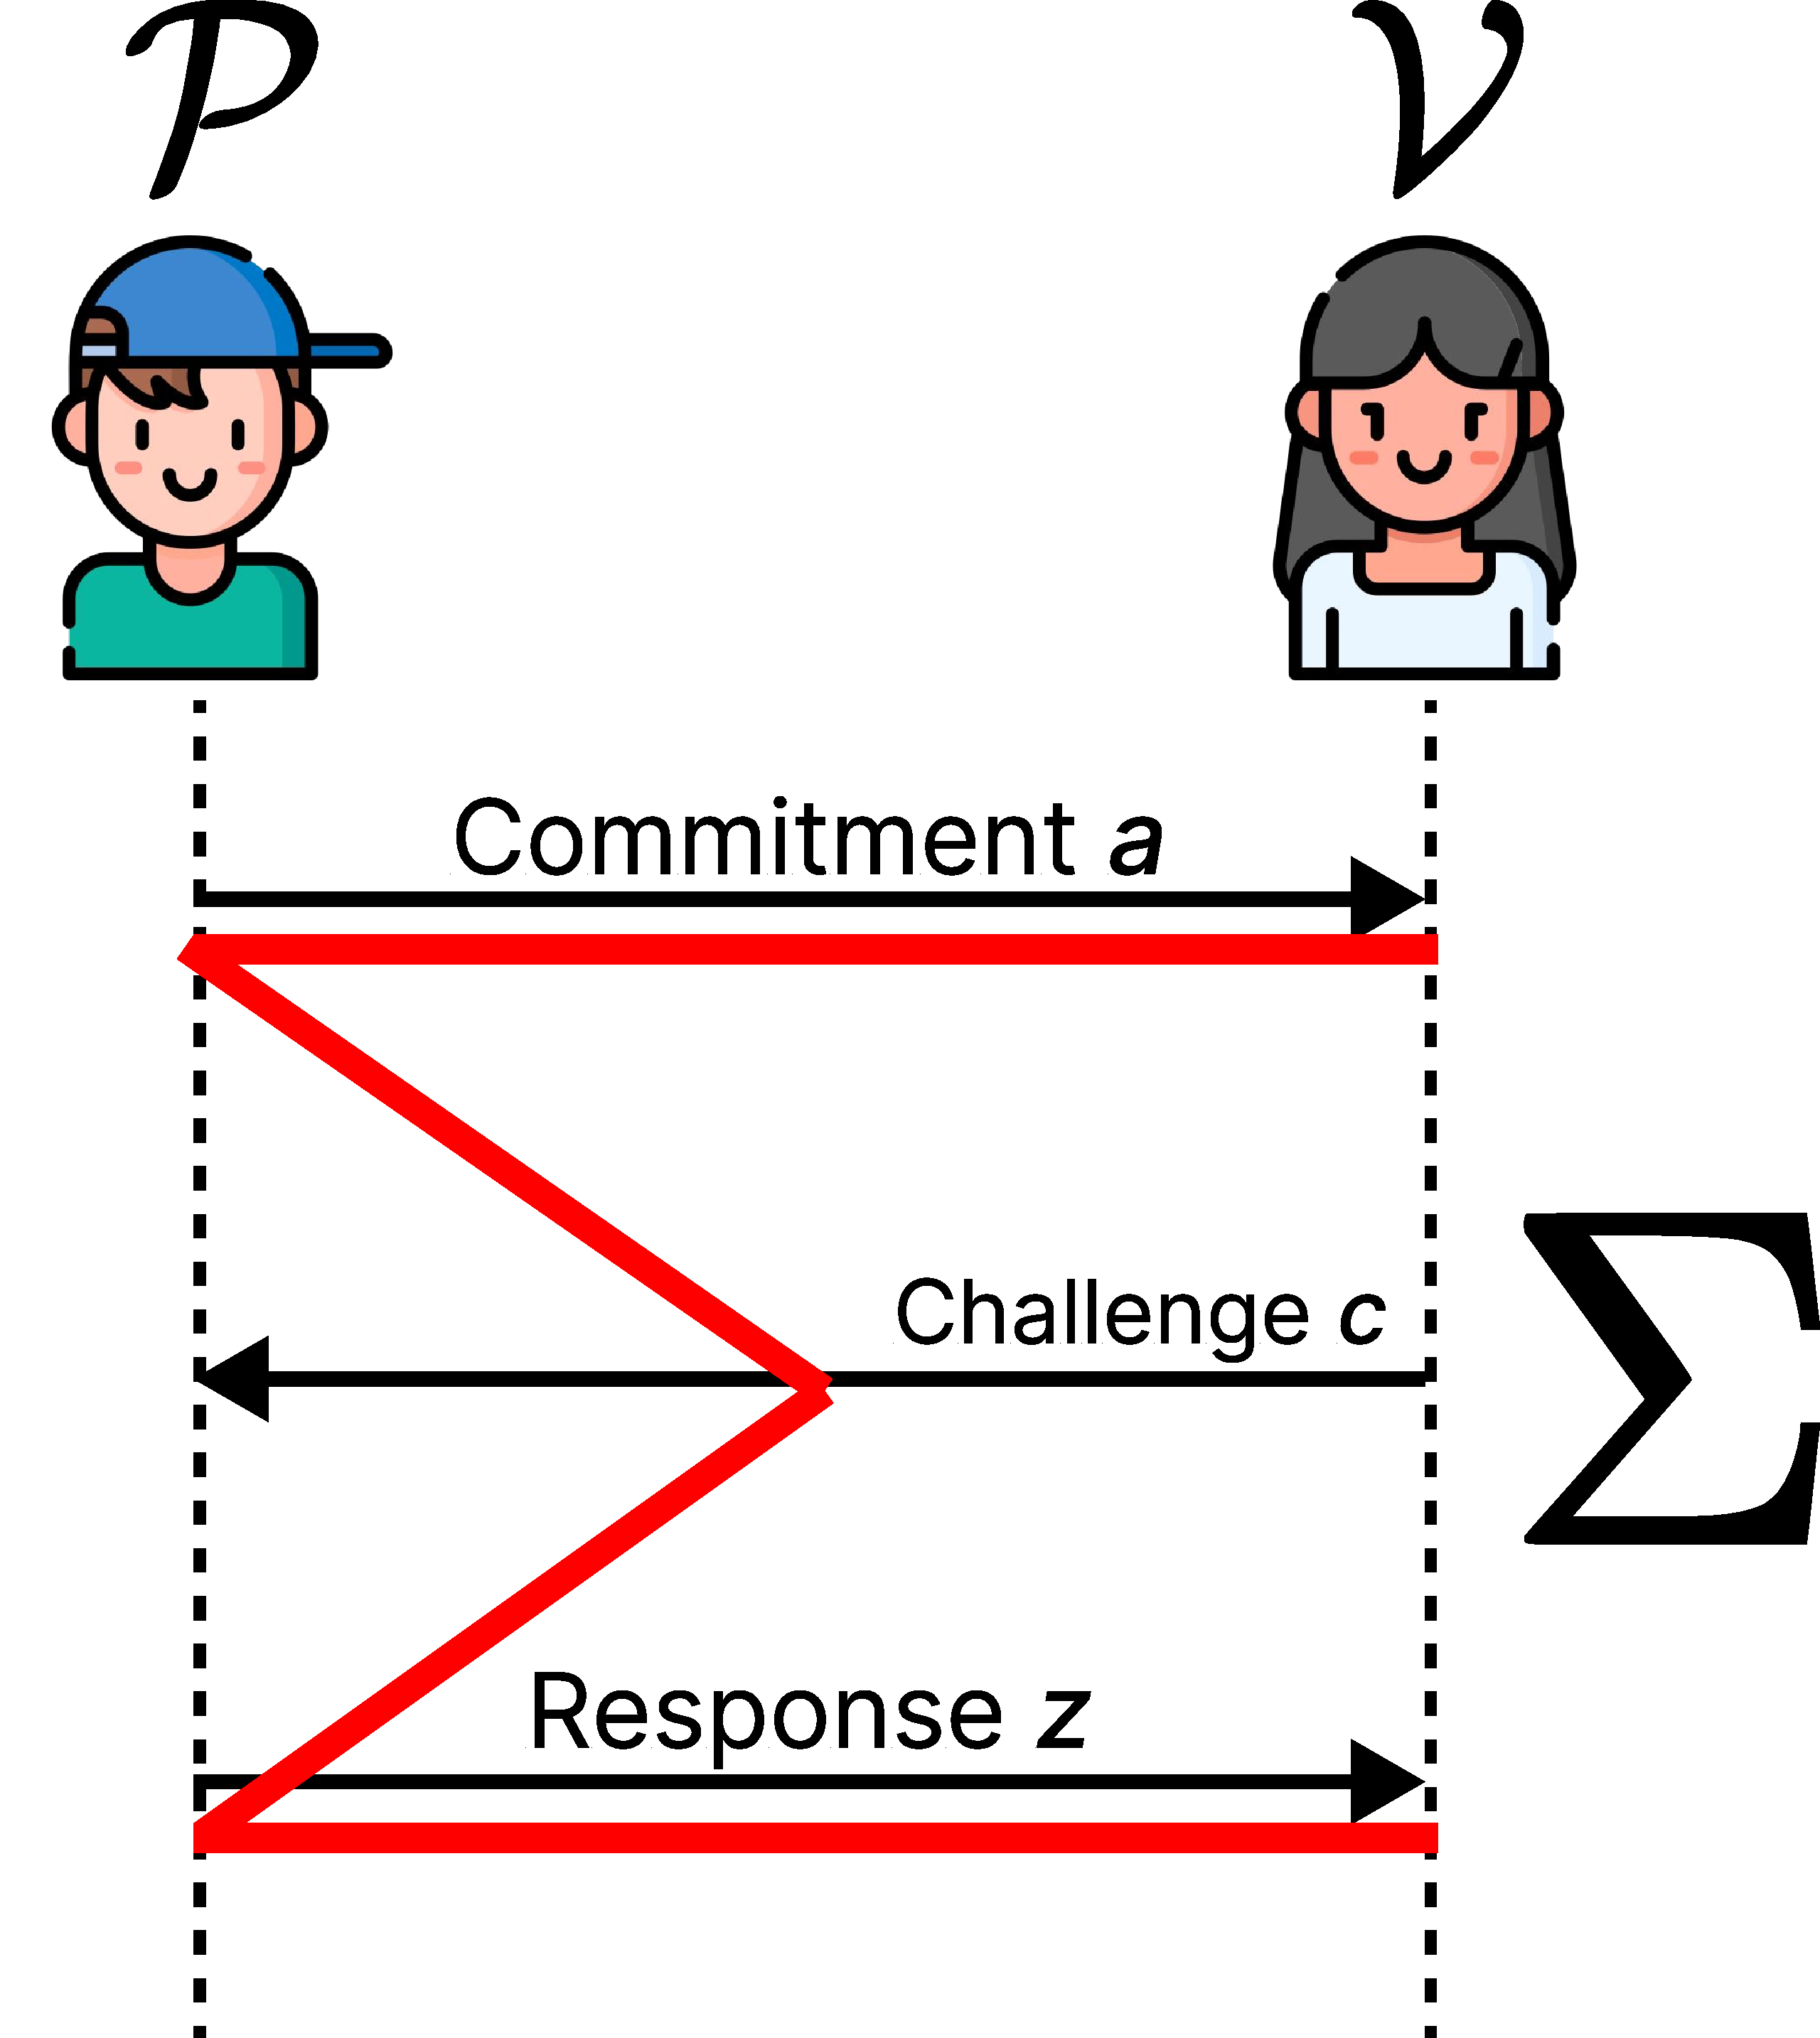
\includegraphics[width=0.3\linewidth]{images/lecture_7/sigma_protocol_illustration.pdf}

    \caption{Sigma Protocol Illustration: the flow of messages between prover $\mathcal{P}$ and verifier $\mathcal{V}$ closely resembles the Greek letter $\Sigma$, which is marked in \textcolor{red}{\textbf{red}} in the Figure.}
    \label{fig:sigma_protocol_illustration}
\end{figure}


\begin{example}
    In particular, for the Schnorr Protocol, the Sigma protocol is defined over the relation $\mathcal{R} \subset \mathcal{X} \times \mathcal{W}$ where:
    \begin{equation*}
        \mathcal{X} = \mathbb{G},\; \mathcal{W} = \mathbb{Z}_q, \; \mathcal{R} = \{(u,\alpha) \in \mathbb{G} \times \mathbb{Z}_q: u = g^{\alpha}\}
    \end{equation*}

    Here, the challenge space $\mathcal{C}$ is a subset of $\mathbb{Z}_q$ (or, typically, the whole set).
\end{example}

Similarly to interactive protocols, Sigma protocols also have a property called \textit{soundness}. However, there is an additional property called \textit{special soundness} that simplifies the general notion of soundness.

\begin{definition}[Special Soundness]
    Let $(\mathcal{P}, \mathcal{V})$ be a $\Sigma$-protocol for $\mathcal{R} \subseteq \mathcal{X} \times \mathcal{Y}$. We that that $(\mathcal{P},\mathcal{V})$ is \textbf{special sound} if there exists a witness extractor $\mathcal{E}$ such that, given statement $x \in \mathcal{X}$ and two accepting conversations $(a,c,z)$ and $(a,c',z')$ (where $c \neq c'$)\footnote{Notice that initial commitments in both conversations are the same!}, the extractor can always efficiently compute the witness $w$ such that $(x,w) \in \mathcal{R}$.
\end{definition}

\begin{example}
    In case of the Schnorr Protocol, the special soundness property is satisfied by the extractor $\mathcal{E}$ that we have constructed in the proof of knowledge. In other words, we can extract the discrete logarithm $\alpha = \mathsf{DLog}_{\mathbb{G}}(u)$ given two accepting conversations $(a,e,\sigma)$ and $(a',e',\sigma')$.
\end{example}

Now, let us consider some more examples of Sigma protocols.

\subsection{More Sigma Protocol Examples}

\subsubsection{Okamoto's Protocol for Representations}

Again, let $\mathbb{G}$ be a cyclic group of prime order $q$ with a generator $g \in \mathbb{G}$ and let $h \in \mathbb{G}$ an arbitrary group element (for example, it might be yet another group generator). While considering Pedersen Commitments, you already encountered form $g^{\alpha}h^{\beta}$. Now, let us generalize this concept a bit.

\begin{definition}
    For $u \in \mathbb{G}$, a \textbf{representation} relative to $g$ and $h$ is a pair $(\alpha,\beta) \in \mathbb{Z}_q \times \mathbb{Z}_q$ such that $u=g^{\alpha}h^{\beta}$.
\end{definition}

\begin{remark}
    Notice that for the given $u$ there are exactly $q$ representations relative to $g$ and $h$. Indeed, $\forall \beta \in \mathbb{Z}_q \, \exists! \alpha \in \mathbb{Z}_q: g^{\alpha} = uh^{-\beta}$. 
\end{remark}

Now, the \textit{Okamoto's Protocol} is a Sigma protocol that allows one party to prove the knowledge of a representation of a given $u \in \mathbb{G}$ relative to $g$ and $h$. In other words, we are working with the relation
\begin{equation*}
    \mathcal{R} = \left\{ (u,(\alpha,\beta)) \in \mathbb{G} \times \mathbb{Z}_q^2: u = g^{\alpha}h^{\beta} \right\}
\end{equation*}

Now, let us describe the protocol.

\begin{definition}[Okamoto's Identification Protocol]
    \textbf{Okamoto's Protocol} consists of two algorithms: $(\mathcal{P}, \mathcal{V})$, where the prover is assumed to know $(u,(\alpha,\beta)) \in \mathcal{R}$ defined above. The protocol is defined as follows:
    \begin{enumerate}
        \item $\mathcal{P}$ computes $\alpha_r \xleftarrow{R} \mathbb{Z}_q, \; \beta_r \xleftarrow{R} \mathbb{Z}_q, \; u_r \gets g^{\alpha_r}h^{\beta_r}$ and sends commitment $u_r$ to $\mathcal{V}$.
        \item $\mathcal{V}$ samples the challenge $c \xleftarrow{R} \mathbb{Z}_q$ and sends $c$ to $\mathcal{P}$.
        \item $\mathcal{P}$ computes $\alpha_z \gets \alpha_r + \alpha c, \beta_z \gets \beta_r + \beta c$ and sends $\mathbf{z} = (\alpha_z,\beta_z)$ to $\mathcal{V}$.
        \item $\mathcal{V}$ checks whether $g^{\alpha_z}h^{\beta_z} = u_r u^c$ and accepts or rejects the proof accordingly.
    \end{enumerate}
\end{definition}

\begin{theorem}
    Okamoto's Protocol is a $\Sigma$-protocol for the relation $\mathcal{R}$ which is Honest-Verifier Zero-Knowledge.
\end{theorem}

\textbf{Part of the proof.} Again, let us show \textit{correctness} and \textit{special soundness} without honest-verifier zero-knowledge properties.

\textit{Completeness.} Suppose indeed that $(u,(\alpha,\beta)) \in \mathcal{R}$. Then, the verification condition can be written as follows:
\begin{equation*}
    g^{\alpha_z}h^{\beta_z} = g^{\alpha_r + \alpha c}h^{\beta_r + \beta c} = g^{\alpha_r}g^{\alpha c}h^{\beta_r}h^{\beta c} = \underbrace{(g^{\alpha_r}h^{\beta_r})}_{=u_r} \cdot (\underbrace{g^{\alpha}h^{\beta}}_{=u})^c = u_r u^c
\end{equation*}

\textit{Special Soundness}. Suppose we are given two accepting conversations: $(u_r,c,(\alpha_z,\beta_z))$ and $(u_r,c',(\alpha_z',\beta_z'))$ and we want to construct an extractor $\mathcal{E}$ which would give us a witness $(\alpha,\beta)$. In this case, we have the following holding:
\begin{equation*}
    g^{\alpha_z}h^{\beta_z} = u_r u^c, \; g^{\alpha_z'}h^{\beta_z'} = u_r u^{c'}
\end{equation*}

We can divide the former by the latter to obtain:
\begin{equation*}
    g^{\alpha_z - \alpha_z'}h^{\beta_z - \beta_z'} = u^{c-c'} = g^{\alpha(c-c')}h^{\beta(c-c')},
\end{equation*}

from which the extractor $\mathcal{E}$ can efficiently compute witness as follows: $\alpha \gets (\alpha_z - \alpha_z')\big/(c-c')$ and $\beta \gets (\beta_z - \beta_z')\big/(c-c')$.

\subsubsection{Chaum-Pedersen protocol for DH-triplets}

As with previous examples, suppose we are given the cyclic group $\mathbb{G}$ or prime order $q$ and generator $g \in \mathbb{G}$. Recall that \textit{the Diffie-Hellman Triple} (or, \textit{DH-triple}) is a triple $(g^{\alpha},g^{\beta},g^{\gamma})$ with $\gamma=\alpha\beta$. Now, this definition is not really convenient for us, so we will reformulate the DH-triple using the proposition below.

\begin{proposition}[Alternative DH-triple Definition]
    $(u,v,w)$ is a DH-triplet iff $\exists \beta \in \mathbb{Z}_q: v = g^{\beta}, w = u^{\beta}$.
\end{proposition}

Now, this makes it easier to define the relation $\mathcal{R}$ for the Chaum-Pedersen protocol:
\begin{equation*}
    \mathcal{R} = \left\{ ((u,v,w), \beta) \in \mathbb{G}^3 \times \mathbb{Z}_q: v = g^{\beta} \wedge w = u^{\beta} \right\}
\end{equation*}

In other words, here we have a witness $\beta \in \mathbb{Z}_q$, while the statement is a triplet $(u,v,w) \in \mathbb{G}^3$. Again, we want to convert this into a Sigma protocol. We do it as follows.

\begin{definition}[Chaum-Pedersen Protocol]
    \textbf{Chaum-Pedersen Protocol} consists of two algorithms: $(\mathcal{P}, \mathcal{V})$, where the prover is assumed to know $(\beta,(u,v,w)) \in \mathcal{R}$ defined above. The protocol is defined as follows:
    \begin{enumerate}
        \item $\mathcal{P}$ computes $\beta_r \xleftarrow{R} \mathbb{Z}_q, \; v_r \xleftarrow{R} g^{\beta_r}, \; w_r \gets u^{\beta_r}$ and sends commitment $(u_r,w_r)$ to $\mathcal{V}$.
        \item $\mathcal{V}$ samples the challenge $c \xleftarrow{R} \mathbb{Z}_q$ and sends $c$ to $\mathcal{P}$.
        \item $\mathcal{P}$ computes $\beta_z \gets \beta_r + \beta c$ and sends $\beta_z$ to $\mathcal{V}$.
        \item $\mathcal{V}$ checks whether two conditions hold: $g^{\beta_z} = v_rv^c$ and $u^{\beta_z} = w_r w^c$, and accepts or rejects the proof accordingly.
    \end{enumerate}
\end{definition}

\begin{theorem}
    Chaum-Pedersen Protocol is a $\Sigma$-protocol for the relation $\mathcal{R}$ which is Honest-Verifier Zero-Knowledge.
\end{theorem}

\textbf{Part of the proof.} As always, let us show \textit{correctness} and \textit{special soundness} without honest-verifier zero-knowledge properties.

\textit{Correctness.} Again, consider the expression $g^{\beta_z}$ more closely:
\begin{equation*}
    g^{\beta_z} = g^{\beta_r + \beta c} = g^{\beta_r}g^{\beta c} = \underbrace{g^{\beta_r}}_{=v_r}(\underbrace{g^{\beta}}_{=v})^c = v_rv^c
\end{equation*}

The similar reasoning can be applied to the second verification condition: indeed, here we have $u^{\beta_z} = u^{\beta_r}(u^{\beta})^c = w_rw^c$

\textit{Special Soundness.} Suppose we are given two accepting conversations: $((u_r,w_r),c,\beta_z)$ and $((u_r,w_r),c',\beta_z')$ and we want to construct an extractor $\mathcal{E}$ which would give us a witness $\beta$. Notice that the following equations hold:
\begin{align*}
    g^{\beta_z} = v_rv^c, \; g^{\beta_z'} = v_rv^{c'}, \\ u^{\beta_z} = w_rw^c, \; u^{\beta_z'} = w_rw^{c'}.
\end{align*}

Divide left equations by the right ones to obtain:
\begin{equation*}
    g^{\beta_z - \beta_z'} = v^{c-c'}, \; u^{\beta_z - \beta_z'} = w^{c-c'}.
\end{equation*}

Consider the first equation. Since $v=g^{\beta}$ we derive $(\beta_z-\beta_z') = \beta(c-c')$, from which $\mathcal{E}$ outputs $\beta = \frac{\beta_z-\beta_z'}{c-c'}$. The same value can be extracted from the second equation.

\subsection{Generalizing Sigma Protocols}

Now, the most interesting part! Probably, you have noticed, that all protocols above (Schnorr, Okamoto, Chaum-Pedersen) have a similar structure. So is there any way to generalize them? The answer is yes and moreover, this done in a very elegant way.

Let $(\mathbb{H}, \oplus)$ and $(\mathbb{T}, \otimes)$ be two finite abelian groups and suppose we have some concrete homomorphism $\psi: \mathbb{H} \to \mathbb{T}$. Moreover, we require that given $t \in \mathbb{T}$, finding the pre-image of $t$ (meaning, finding some $h \in \mathbb{H}$ such that $\psi(h)=t$) is computationally hard. Suppose $\mathcal{F}$ is a set of all homomorphisms from $\mathbb{H}$ to $\mathbb{T}$ (sometimes denoted as $\mathsf{Hom}(\mathbb{H}, \mathbb{T})$). Now, define the following relation:
\begin{equation*}
    \mathcal{R} = \left\{ ((t,\psi), h) \in (\mathbb{T} \times \mathcal{F}) \times \mathbb{H}: \psi(h) = t \right\}
\end{equation*}

And now the prover $\mathcal{P}$ wants to convince the verifier $\mathcal{V}$ that he knows the witness $h$ to the statement $(t,\psi)$. 
\begin{proposition}
    Now, why does this generalize the previous protocols? Well, let us consider all previous examples:
    \begin{itemize}
        \item \textbf{Schnorr Protocol:} Here we have $\mathbb{H} = \mathbb{Z}_q$, $\mathbb{T} = \mathbb{G}$, and $\psi: \mathbb{Z}_q \to \mathbb{G}$ is defined as $\psi(\alpha) = g^{\alpha}$. Moreover, here $\psi$ is an isomorphism!
        \item \textbf{Okamoto Protocol:} Here we have $\mathbb{H} = \mathbb{Z}_q^2$, $\mathbb{T} = \mathbb{G}$, and $\psi: \mathbb{Z}_q^2 \to \mathbb{G}$ is defined as $\psi(\alpha,\beta) = g^{\alpha}h^{\beta}$. It is also quite easy to see that $\psi$ is a homomorphism:
        \begin{equation*}
            \begin{aligned}
                &\psi((\alpha,\beta) + (\alpha',\beta')) = \psi(\alpha+\alpha',\beta+\beta') = g^{\alpha+\alpha'}h^{\beta+\beta'} = \\ 
                &= g^{\alpha}h^{\beta}g^{\alpha'}h^{\beta'} = \psi(\alpha,\beta)\psi(\alpha',\beta')                
            \end{aligned}
        \end{equation*}
        \item \textbf{Chaum-Pedersen Protocol:} Here we have $\mathbb{H} = \mathbb{Z}_q$, $\mathbb{T} = \mathbb{G}^2$, and $\psi: \mathbb{Z}_q \to \mathbb{G}^2$ is defined as $\psi(\beta) = (g^{\beta},u^{\beta})$. Again, it is easy to see that $\psi$ is a homomorphism.
    \end{itemize}
\end{proposition}

Now, we formulate the general Sigma protocol for the relation $\mathcal{R}$ over homomorphism.

\begin{definition}[Sigma Protocol for the pre-image of a homomorphism]
    The protocol consists of two algorithms: $(\mathcal{P}, \mathcal{V})$, where the prover is assumed to know the witness $h \in \mathbb{H}$ defined above. The protocol is defined as follows:
    \begin{enumerate}
        \item $\mathcal{P}$ computes $h_r \xleftarrow{R} \mathbb{H}, t_r \gets \psi(h_r) \in \mathbb{T}$ and sends $t_r$ to the verifier $\mathcal{V}$.
        \item $\mathcal{V}$ samples the challenge $c \xleftarrow{R} \mathcal{C} \subset \mathbb{Z}$ from the challenge space and sends $c$ to $\mathcal{P}$.
        \item $\mathcal{P}$ computes $h_z \gets h_r \oplus h\cdot c$ and sends $h_z$ to $\mathcal{V}$.
        \item $\mathcal{V}$ checks whether $\psi(h_z) = t_r \otimes t^c$, and accepts or rejects the proof accordingly.
    \end{enumerate}
\end{definition}

\subsection{Combining Sigma Protocols}

Now, suppose we have the Sigma interactive protocol $(\mathcal{P}_0,\mathcal{V}_0)$ for one relation $\mathcal{R}_0 \subseteq \mathcal{W}_0 \times \mathcal{X}_0$ and another Sigma interactive protocol $(\mathcal{P}_1,\mathcal{V}_1)$ for another relation $\mathcal{R}_1 \subseteq \mathcal{W}_1 \times \mathcal{X}_1$. Now, we want to combine these two protocols into a single one. Namely, we want our prover to be able to convince the verifier that:
\begin{enumerate}
    \item He knows the witnesses $w_0,w_1$ to both statements $x_0,x_1$.
    \item He knows the witness $w \in \mathcal{W}_0 \cup \mathcal{W}_1$ to either statement $x_0$ or $x_1$.
\end{enumerate}

Among two, the second one is a bit more interesting since it allows us to prove the knowledge of a witness to either of the statements. This is called the \textit{OR-composition} of Sigma protocols.

\subsubsection{The AND Sigma Protocol}

Now, let the prover $\mathcal{P}$ prove the witness knowledge of the following relation:
\begin{equation*}
    \scalebox{0.85}{$
        \mathcal{R}_{\text{AND}} = \left\{ ((x_0,x_1), (w_0,w_1)) \in (\mathcal{X}_0 \times \mathcal{X}_1) \times (\mathcal{W}_0 \times \mathcal{W}_1): (w_0,x_0) \in \mathcal{R}_0 \wedge (w_1,x_1) \in \mathcal{R}_1 \right\}
    $}
\end{equation*}

We define the following protocol.

\begin{definition}[The AND Sigma Protocol]
    Define a pair of algorithms $(\mathcal{P},\mathcal{V})$ which are run as follows:
    \begin{enumerate}
        \item The prover $\mathcal{P}$ runs $\mathcal{P}_0(w_0,x_0)$ to get commitment $a_0$ and runs $\mathcal{P}_1(w_1,x_1)$ to get $a_1$ and sends the pair $\mathbf{a} = (a_0,a_1)$ to $\mathcal{V}$.
        \item The verifier computes the challenge $c \xleftarrow{R} \mathcal{C}$ and sends it to $\mathcal{P}$.
        \item The prover feeds provers $\mathcal{P}_0(w_0,x_0)$ and $\mathcal{P}_1(w_1,x_1)$ with the challenge to get responses $z_0$ and $z_1$, respectively. He then sends $\mathbf{z} = (z_0,z_1)$ to $\mathcal{V}$.
        \item The verifier checks whether both $\mathcal{V}_0(a_0,c,z_0)$ and $\mathcal{V}_1(a_1,c,z_1)$ pass.
    \end{enumerate}
\end{definition}

However, such protocol is not very interesting since what we did essentially is just running two protocols separately: one for $(\mathcal{P}_0,\mathcal{V}_0)$, and the other for $(\mathcal{P}_1,\mathcal{V}_1)$. The only difference is that we use the single challenge for both protocols.

\subsubsection{The OR Sigma Protocol}

The less trivial example is the following: define the relation
\begin{equation*}
    \scalebox{0.85}{$
    \mathcal{R}_{\text{OR}} = \left\{ ((x_0, x_1), (w, b)) \in (\mathcal{X}_0 \times \mathcal{X}_1) \times ((\mathcal{W}_0 \cup \mathcal{W}_1) \times \{0,1\}): (x, w_b) \in \mathcal{R}_b \right\}
    $}
\end{equation*}

Here, the statement is $x_0$ and $x_1$, but the witness is the witness $w$ to either $x_0$ or $x_1$, and the bit $b \in \{0,1\}$, marking to which of the statement $w$ belongs to. That being said, $w$ might be from either set $\mathcal{W}_0$ or $\mathcal{W}_1$: that is why we say that $w \in \mathcal{W}_0 \cup \mathcal{W}_1$.

To make the interactive protocol work, we add one more assumption about both relations $\mathcal{R}_0$ and $\mathcal{R}_1$. Suppose that the challenge space $\mathcal{C} \subseteq \{0,1\}^{\ell}$. This assumption is not very strong as typically $\mathcal{C}$ is some subspace of integers and thus decomposing some $c \in \mathcal{C}$ into the fixed-length bit representation is a trivial task.

Now, we describe the algorithm.

\begin{definition}[The OR Sigma Protocol]
    Define a pair of algorithms $(\mathcal{P},\mathcal{V})$ for relation $\mathcal{R}_{\text{OR}}$ with $b^* := 1-b$ as follows:
    \begin{enumerate}
        \item The prover chooses a random challenge $c_{b^*} \xleftarrow{R} \mathcal{C}$ and generates random commitment and response $(a_{b^*}, z_{b^*})$ that form a valid accepting conversation $(a_{b^*}, c_{b^*}, z_{b^*})$ (essentially, the prover runs the simulator $(a_{b^*}, z_{b^*}) \xleftarrow{R} \mathsf{Sim}_{b^*}(x_{b^*}, c_{b^*})$). Then, $\mathcal{P}$ also runs $\mathcal{P}_b(x_b, w)$ to get a valid commitment $a_b$ and sends $(a_0,a_1)$ to $\mathcal{V}$.
        \item The verifier sends a random challenge $c \xleftarrow{R} \mathcal{C} \subseteq \{0,1\}^{\ell}$.
        \item The prover XORs both challenges: $c_b \gets c \oplus c_{b^*}$. Then it feeds the challenge $c_b$ to the prover $\mathcal{P}_b(x_b,w)$ to get the responses $z_b$ ($b \in \{0,1\}$) and sends $(c_0,z_0,z_1)$ to $\mathcal{V}$.
        \item Verifier computes $c_1 \gets c \oplus c_0$ and checks that both verifications $\mathcal{V}_0(a_0,c_0,z_0)$ and $\mathcal{V}_1(a_1,c_1,z_1)$ pass.
    \end{enumerate}
\end{definition}

\subsection{Exercises}

\begin{tcolorbox}[colback=gray!10!white,fonttitle=\bfseries,colframe=purple!80!black,title=Exercises 1-5. In search of correct Schnorr's Identification Protocol\ldots]
    \textit{You are given the protocol and five ways to implement it. Most of them lack the crucial properties. For each attempt, you need to determine whether the protocol is correct and, if not, specify which of the properties are violated.}
    \vspace{10px}
 
    Recall, that given the cyclic group $\mathbb{G}$ of order $q$, the prover wants to convince the verifier that he knows the discrete logarithm $\alpha$ of $h \in \mathbb{G}$ with respect to the generator $g \in \mathbb{G}$ (so that $g^{\alpha}=h$).

    Here are five attempts to construct the protocol:

    \textcolor{purple!80!black}{\textbf{Attempt 1.}} Prover sends witness $\alpha$ to the verifier. Verifier checks whether $h = g^{\alpha}$.

    \textcolor{purple!80!black}{\textbf{Attempt 2.}} Prover chooses random $r \xleftarrow{R} \mathbb{Z}_q$ and sends $a \gets \alpha + r$ to the verifier. Verifier checks whether $h = g^a$.

    \textcolor{purple!80!black}{\textbf{Attempt 3.}} Prover chooses random $r \xleftarrow{R} \mathbb{Z}_q$, calculates $a \gets \alpha + r$ and sends both $(a,r)$ to the verifier. Verifier checks whether $g^r h = g^a$.

    \textcolor{purple!80!black}{\textbf{Attempt 4.}} Prover chooses random $r \xleftarrow{R} \mathbb{Z}_q$, calculates $a \gets g^r, z \gets \alpha+r$ and sends $(a,z)$ to the verifier. Verifier checks whether $a \cdot h = g^z$.

    \textcolor{purple!80!black}{\textbf{Attempt 5.}} Prover chooses random $r \xleftarrow{R} \mathbb{Z}_q$, calculates $a \gets g^r$, and sends $a$ to the verifier. Verifier chooses $e \xleftarrow{R} \mathbb{Z}_q$ and sends to the prover. Prover calculates $z \gets \alpha e + r$ and sends to the prover. Verifier checks whether $a \cdot h^e = g^z$.

    \vspace{10px}

    Below, mark whether the properties of \textit{completeness}, \textit{soundness}, and \textit{zero-knowledge} hold for each attempt.

    \begin{center}
    \begin{tabular}{ |l|c|c|c|c|c| } 
        \hline
        \textbf{Attempt \#} & \textbf{1} & \textbf{2} & \textbf{3} & \textbf{4} & \textbf{5} \\ \hline
        \textbf{Completeness} holds? & \cmark/\xmark & \cmark/\xmark & \cmark/\xmark & \cmark/\xmark & \cmark/\xmark \\ \hline
        \textbf{Soundness} holds? & \cmark/\xmark & \cmark/\xmark & \cmark/\xmark & \cmark/\xmark & \cmark/\xmark \\ \hline
        \textbf{Zero-Knowledge} holds? & \cmark/\xmark & \cmark/\xmark & \cmark/\xmark & \cmark/\xmark & \cmark/\xmark\\ \hline
    \end{tabular}
    \end{center}
\end{tcolorbox}

\begin{tcolorbox}[breakable, colback=gray!10!white,fonttitle=\bfseries,colframe=purple!80!black,title=Exercises 6-10. Non-Interactive Chaum-Pedersen Protocol.]
    \textit{This section explores how to make the previously considered Chaum-Pedersen protocol non-interactive. Fill in the gaps in the following text with the correct statements.}
    \vspace{10px}

    Recall that the Chaum-Pedersen protocol allows the prover $\mathcal{P}$ to convince the skeptical verifier $\mathcal{V}$ that the given triplet $(u,v,w) \in \mathbb{G}^3$ is a Diffie-Hellman (DH) triplet in the cyclic group $\mathbb{G}$ of prime order $q$ with a generator $g \in \mathbb{G}$, meaning that $u=g^{\alpha},v=g^{\beta},w=g^{\alpha\beta}$ for some $\alpha,\beta \in \mathbb{Z}_q$. However, instead of making $(\alpha,\beta)$ as a witness, observe that $\beta$ is sufficient. Indeed, if $u=g^{\alpha},v=g^{\beta}$, then $w=\boxed{\textcolor{purple!80!black}{\textbf{6}}}$. Thus, the relation is:
    \begin{equation*}
        \mathcal{R} = \left\{ ((u,v,w), \beta) \in \mathbb{G}^3 \times \mathbb{Z}_q: \boxed{\textcolor{purple!80!black}{\textbf{7}}} \right\}
    \end{equation*}

    Now, we apply the \textit{Fiat-Shamir Transformation}. Recall that prover, instead of getting the random challenge $c \xleftarrow{R} \mathcal{C} \subset \mathbb{Z}_q$ from the verifier interactively, calculates it as the hash function from the public statement $(u,v,w)$ and the prover's commitment. For that reason, define the non-interactive proof system $\Phi = (\mathsf{Gen}, \mathsf{Verify})$ as follows:
    \begin{itemize}
        \item $\mathsf{Gen}$: On input $(u,v,w) \in \mathbb{G}^3$, 
        \begin{enumerate}
            \item Sample $\beta_r \xleftarrow{R} \mathbb{Z}_q$ and compute the commitment $\boxed{\textcolor{purple!80!black}{\textbf{8}}}$.
            \item Use the hash function $\boxed{\textcolor{purple!80!black}{\textbf{9}}}$ to get the challenge $c \gets \boxed{\textcolor{purple!80!black}{\textbf{10}}}$.
            \item Compute response $\beta_z \gets \beta_r + \beta c$ and output commitment $(v_r,w_r)$ and $\beta_z$ as a proof $\pi$.
        \end{enumerate}
        \item $\mathsf{Verify}$: Upon receiving statement $(u,v,w)$ and a proof $\pi=(v_r,w_r,\beta_z)$, the verifier:
        \begin{enumerate}
            \item Recomputes the challenge $c$ using the hash function.
            \item Accepts if and only if $g^{\beta_z} = v_r v^c$ and $u^{\beta_z} = w_r w^c$.
        \end{enumerate}
    \end{itemize}

    \begin{center}
        \begin{tabular}{p{5cm}p{5cm}}
            % Exercise 3
            \textbf{Exercise 6.}
            \begin{enumerate}[A)]
                \item $v^{\beta}$
                \item $u^{\beta}$
                \item $vu$
                \item $v^u$
                \item $v^{\beta}u$
            \end{enumerate} &   
            \textbf{Exercise 7.}
            \begin{enumerate}[A)]
                \item $v = g^{\beta}$ and $w = vu$
                \item $v = g^{\beta}$ and $w = v^{\beta}$
                \item $v = g^{\beta}$ and $w = u^{\beta}$
                \item $u = g^{\beta}$ and $w = u^{\beta}$
                \item $u/w = g^{\beta}$
            \end{enumerate} \\

            \textbf{Exercise 8.}
            \begin{enumerate}[A)]
                \item $(v_r,w_r) = (g^{\beta_r},g^{\beta_r\beta})$
                \item $(v_r,w_r) = (g^{\beta_r},w^{\beta_r})$
                \item $(v_r,w_r) = (g^{\beta_r},u^{\beta_r})$
                \item $(v_r,w_r) = (g^{\beta},g^{\beta_r})$
                \item $(v_r,w_r) = (g^{\beta},g^{\beta_r}g^{\beta})$
            \end{enumerate}
            &
            \textbf{Exercise 9.}
            \begin{enumerate}[A)]
                \item $H: \mathbb{G}^3 \times \mathbb{G}^2 \to \mathcal{C}$
                \item $H: \mathbb{G}^3 \times (\mathbb{G} \times \mathbb{Z}_q) \to \mathcal{C}$
                \item $H: \mathbb{G}^3 \to \mathcal{C}$
                \item $H: \mathbb{G}^3 \times \mathbb{Z}_q \to \mathcal{C}$
                \item $H: \mathbb{G}^2 \times \mathbb{Z}_q \to \mathcal{C}$
            \end{enumerate} 
            \\

            \textbf{Exercise 10.}
            \begin{enumerate}[A)]
                \item $H((u,v,w),(v_r,w_r))$
                \item $H((u,v,w),(v_r,\beta_r))$
                \item $H(u,v,w)$
                \item $H((u,v,w),\beta_r)$
                \item $H((v_r,w_r),\beta_r)$
            \end{enumerate} 
        \end{tabular}
    \end{center}
\end{tcolorbox}

\end{document}